\chapter{Additional Figures}\label{ch:additional_qual}

\begin{figure}[htb]
\centering
\begin{subfigure}{0.45\textwidth}
    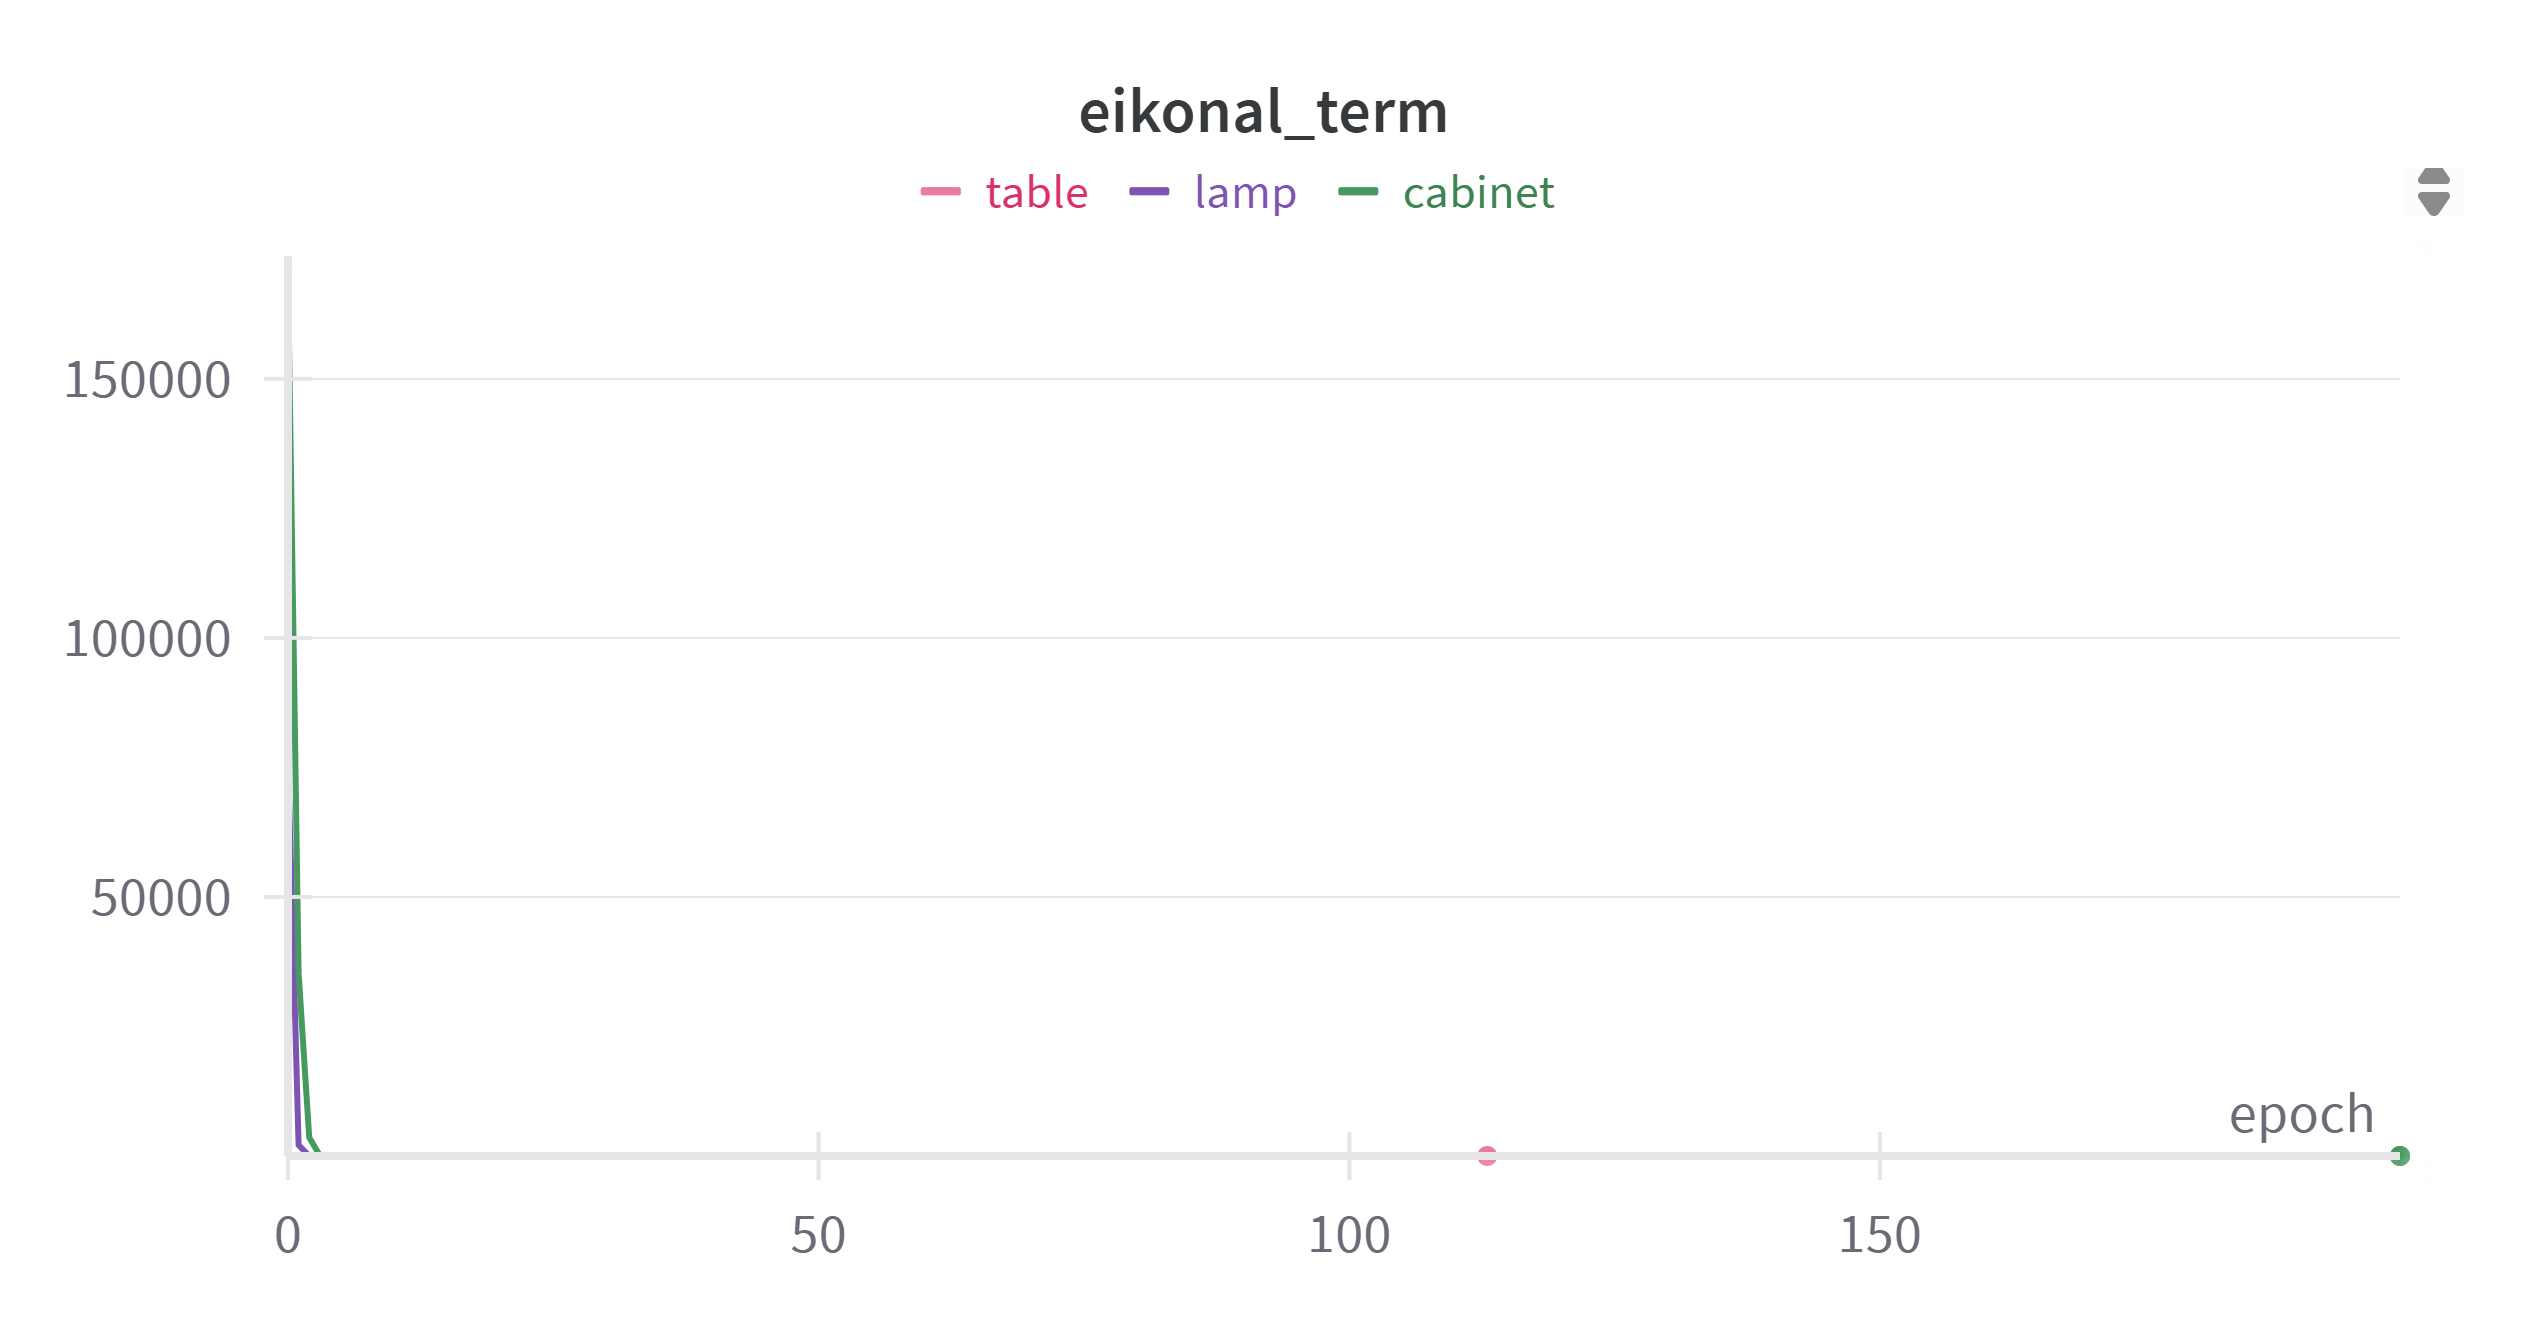
\includegraphics[width=\linewidth]{figures/hessianfail/eikonal.png}
    \caption{Eikonal loss}
\end{subfigure}
\hfill
\begin{subfigure}{0.45\textwidth}
    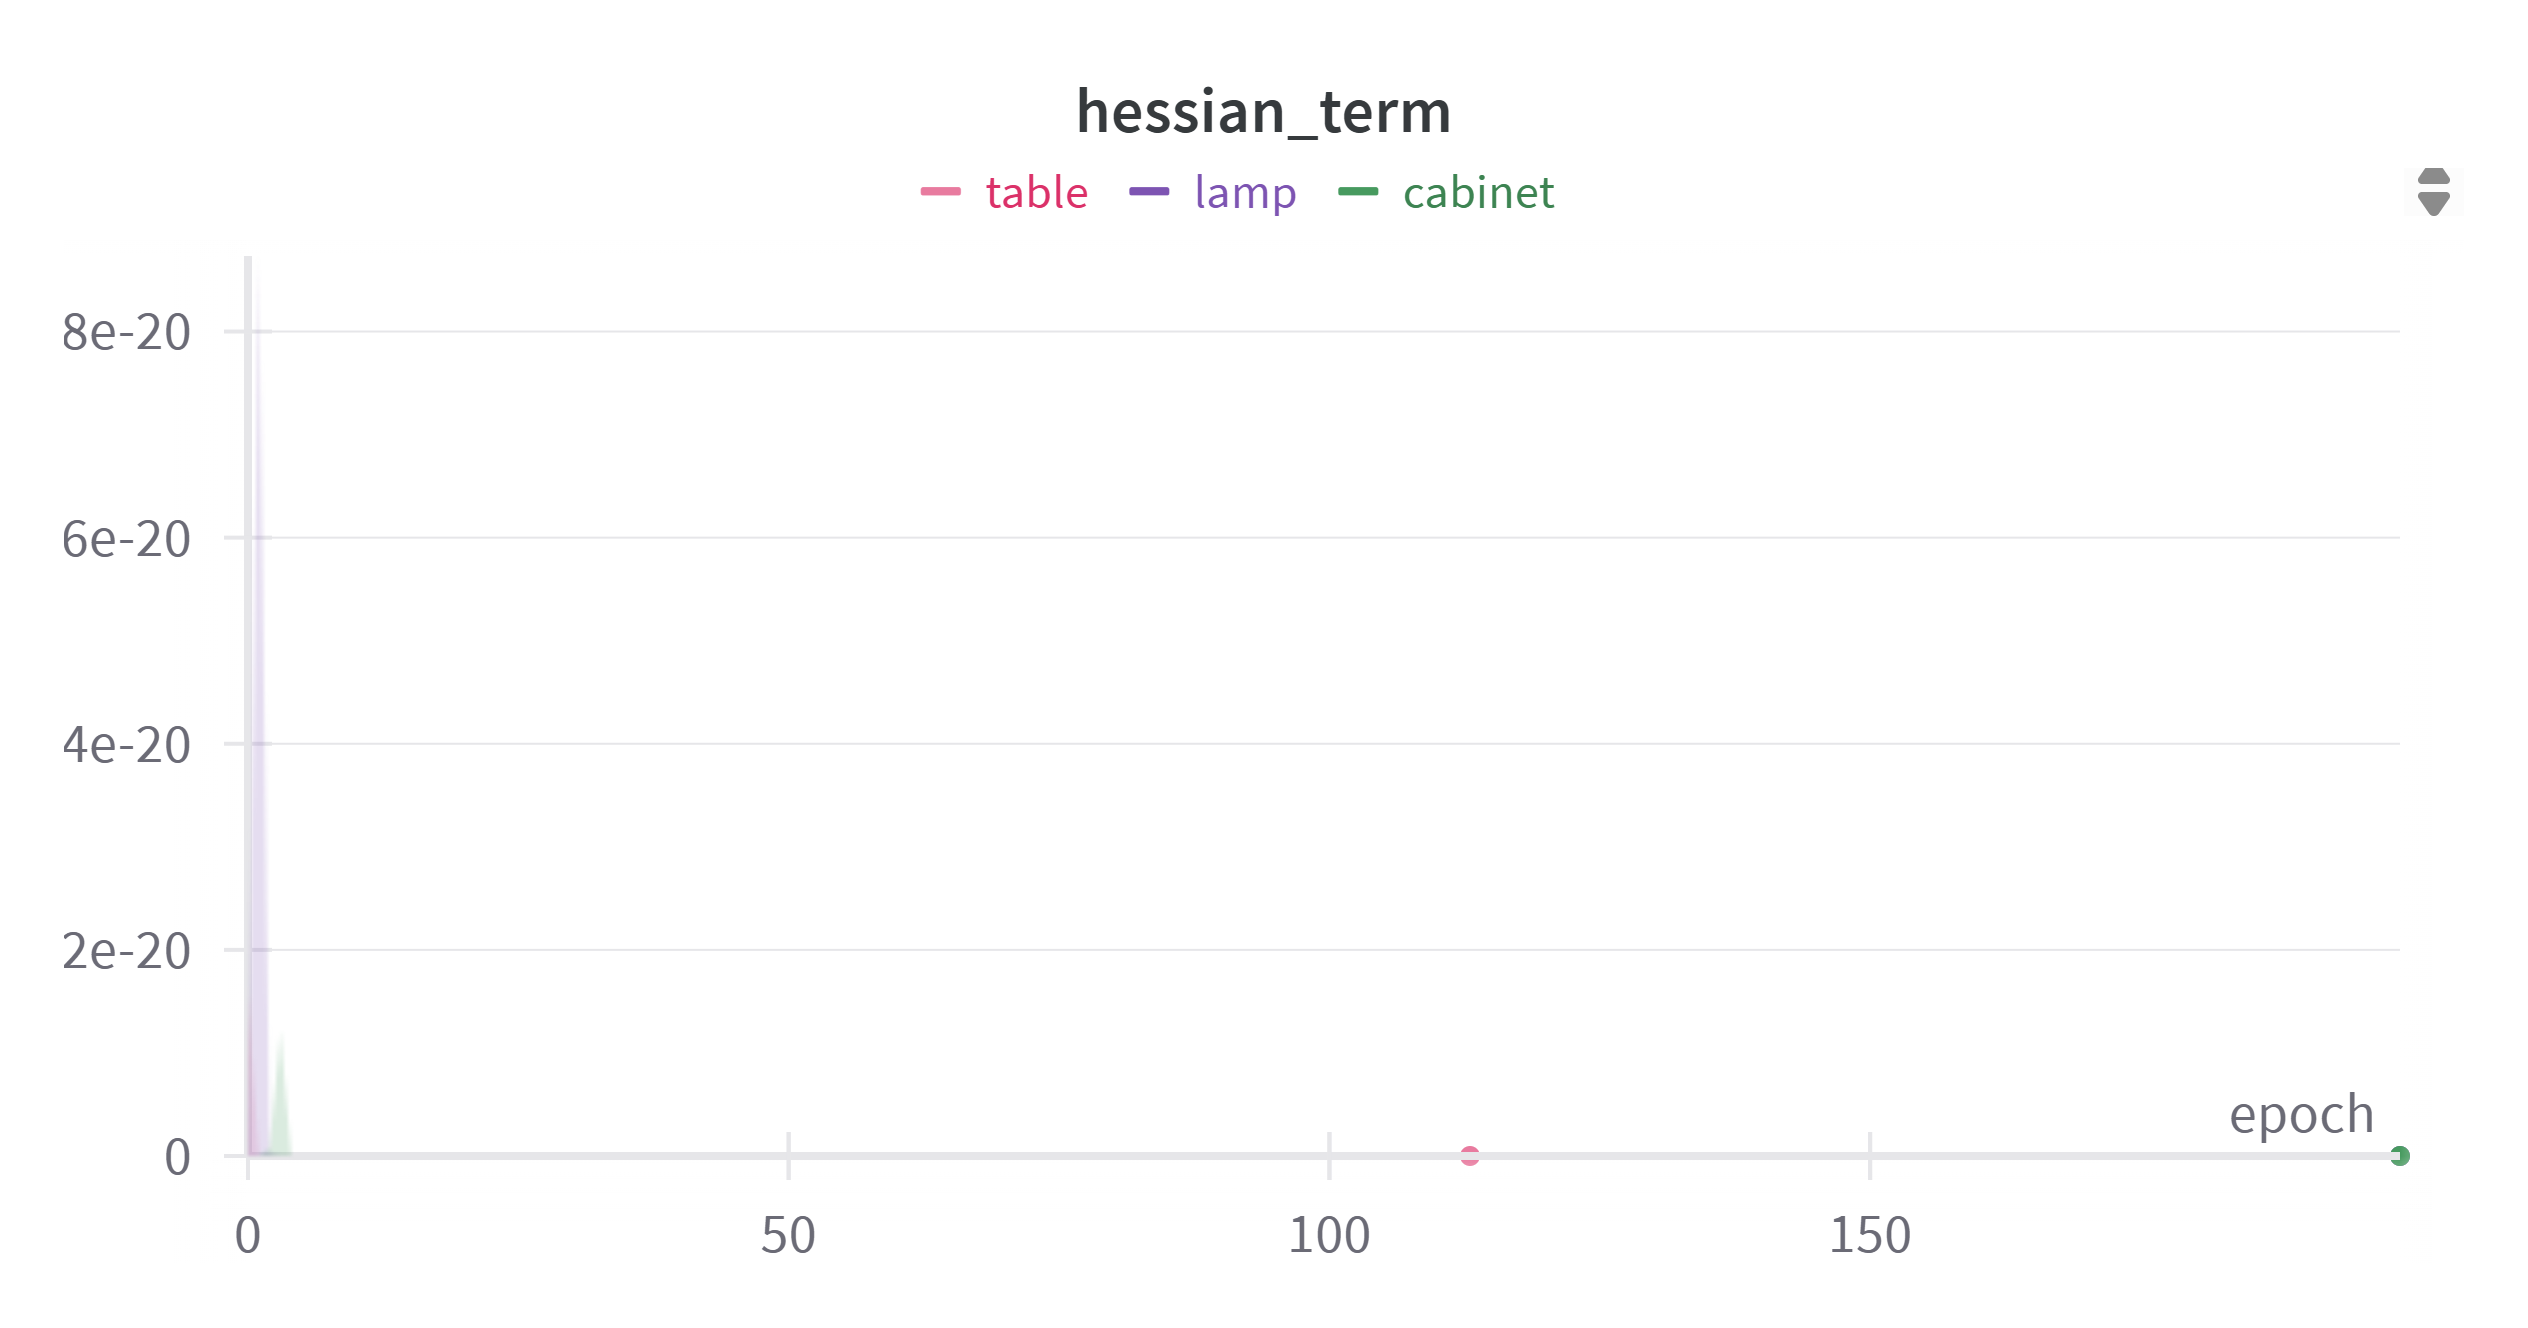
\includegraphics[width=\linewidth]{figures/hessianfail/hessian.png}
    \caption{Determinant of Hessian}
\end{subfigure}
\caption{Plots showing failure to learn conditional implicit representation from partial cloud input due to vanishing gradients.}
\label{fig:hessianfail}
\end{figure}

\begin{figure}[htb]
\centering
\begin{subfigure}{0.315\textwidth}
    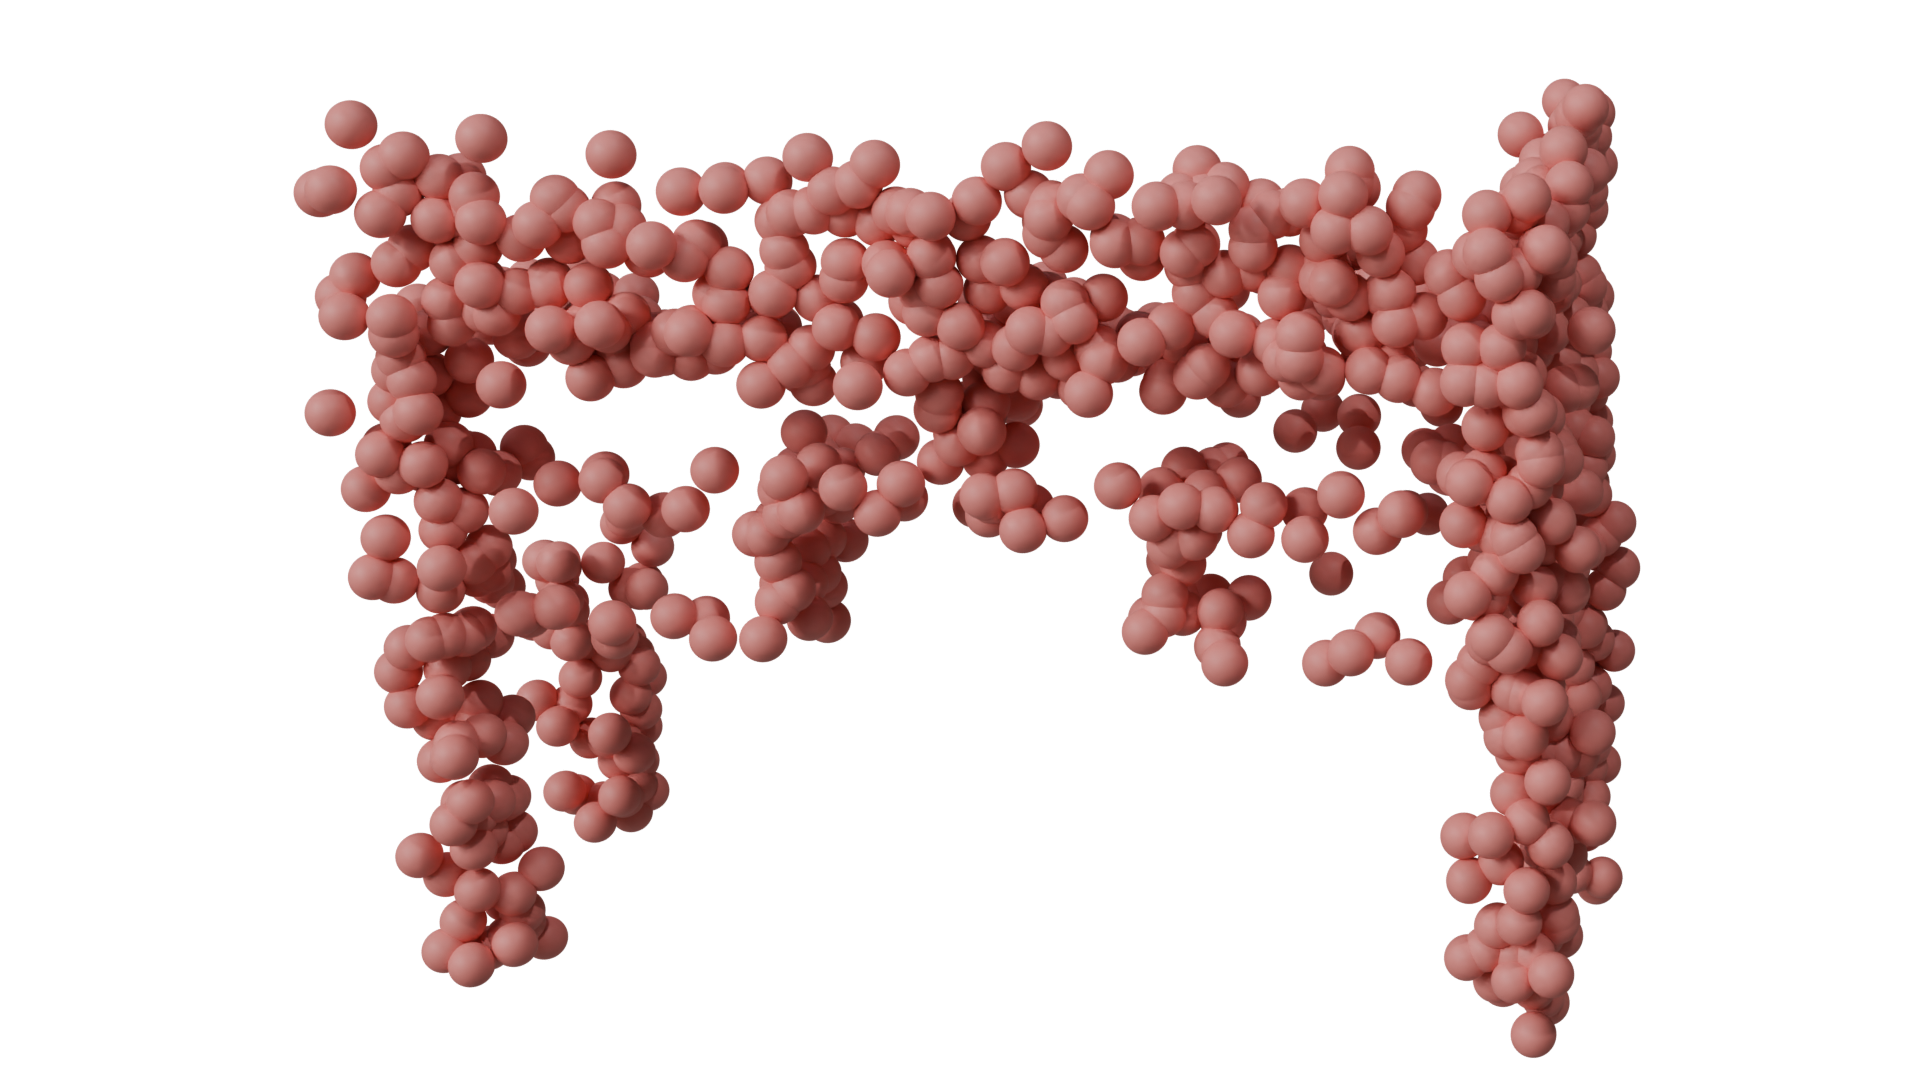
\includegraphics[width=\linewidth]{figures/gp/t1pgp.png}
    \caption{Partial cloud}
\end{subfigure}
\hfill
\begin{subfigure}{0.315\textwidth}
    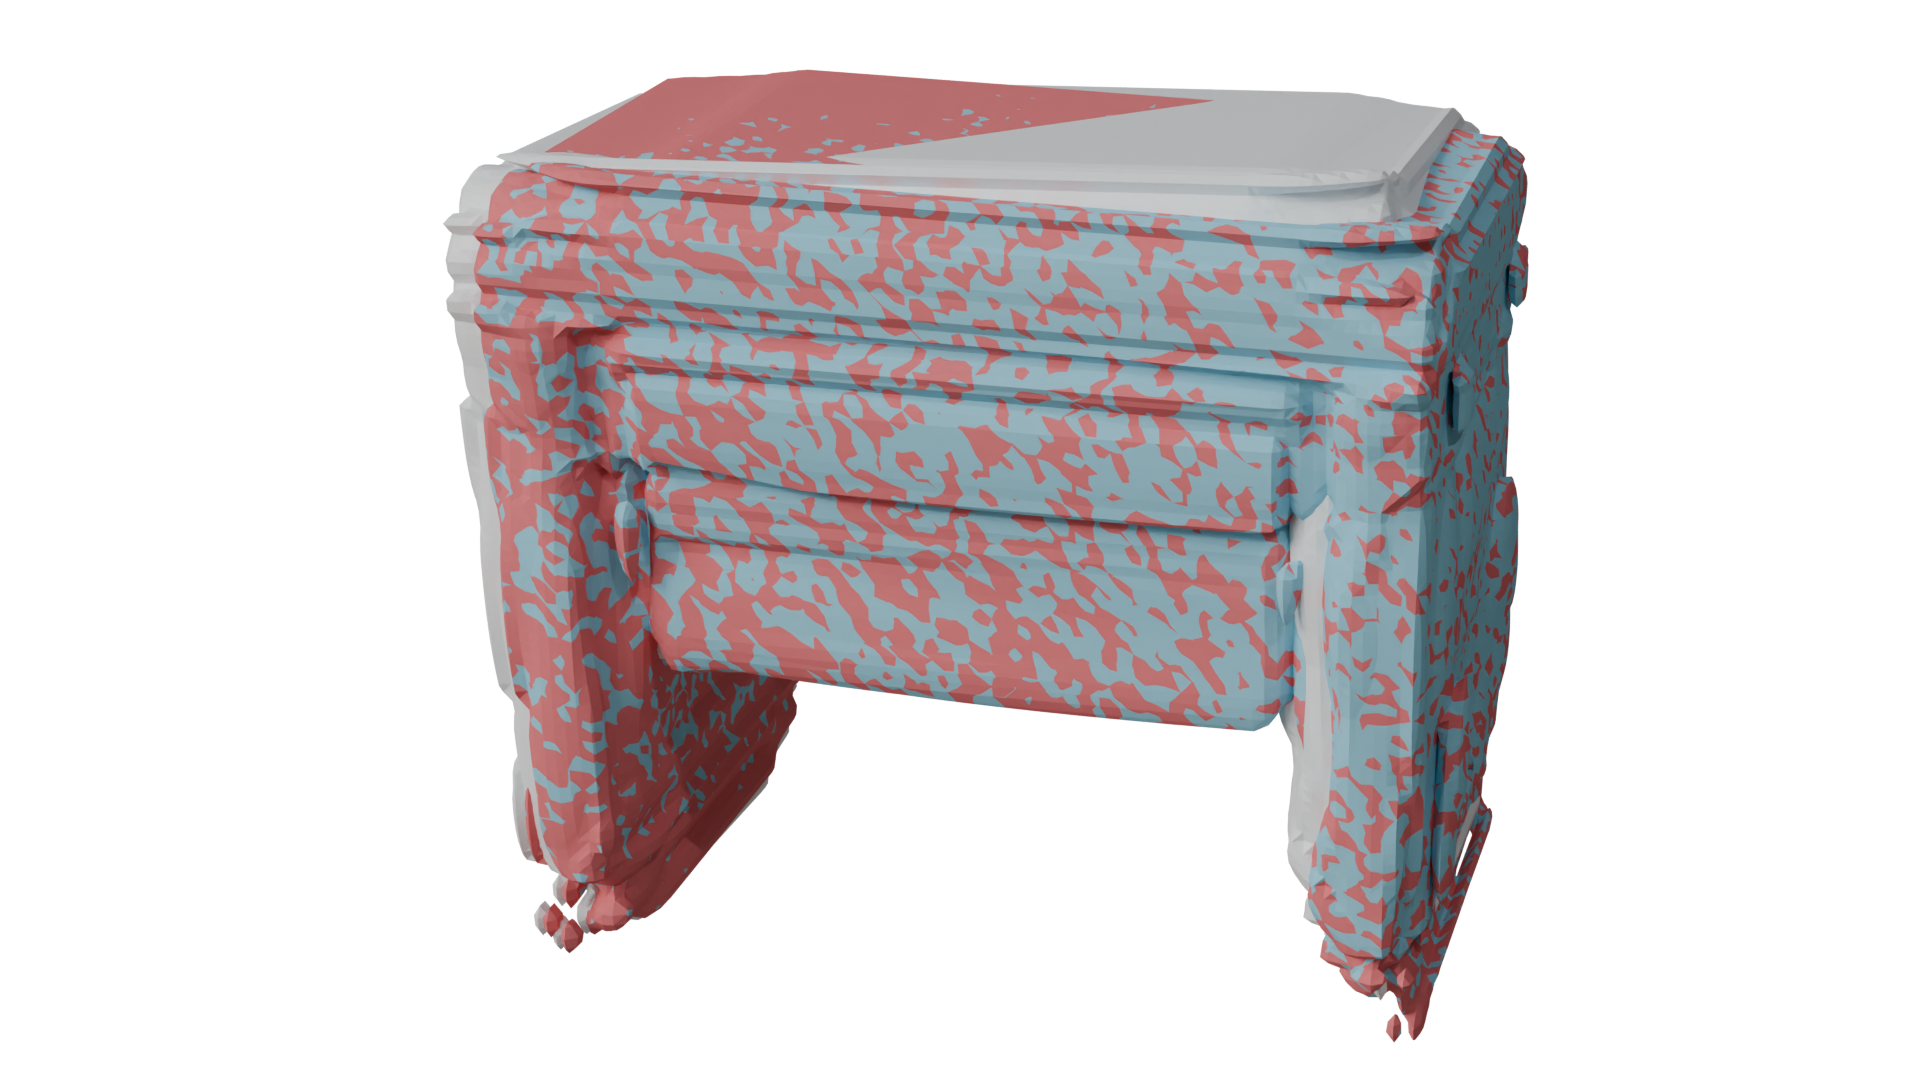
\includegraphics[width=\linewidth]{figures/gp/t1gp+-.png}
    \caption{Recon 1}
\end{subfigure}
\hfill
\begin{subfigure}{0.315\textwidth}
    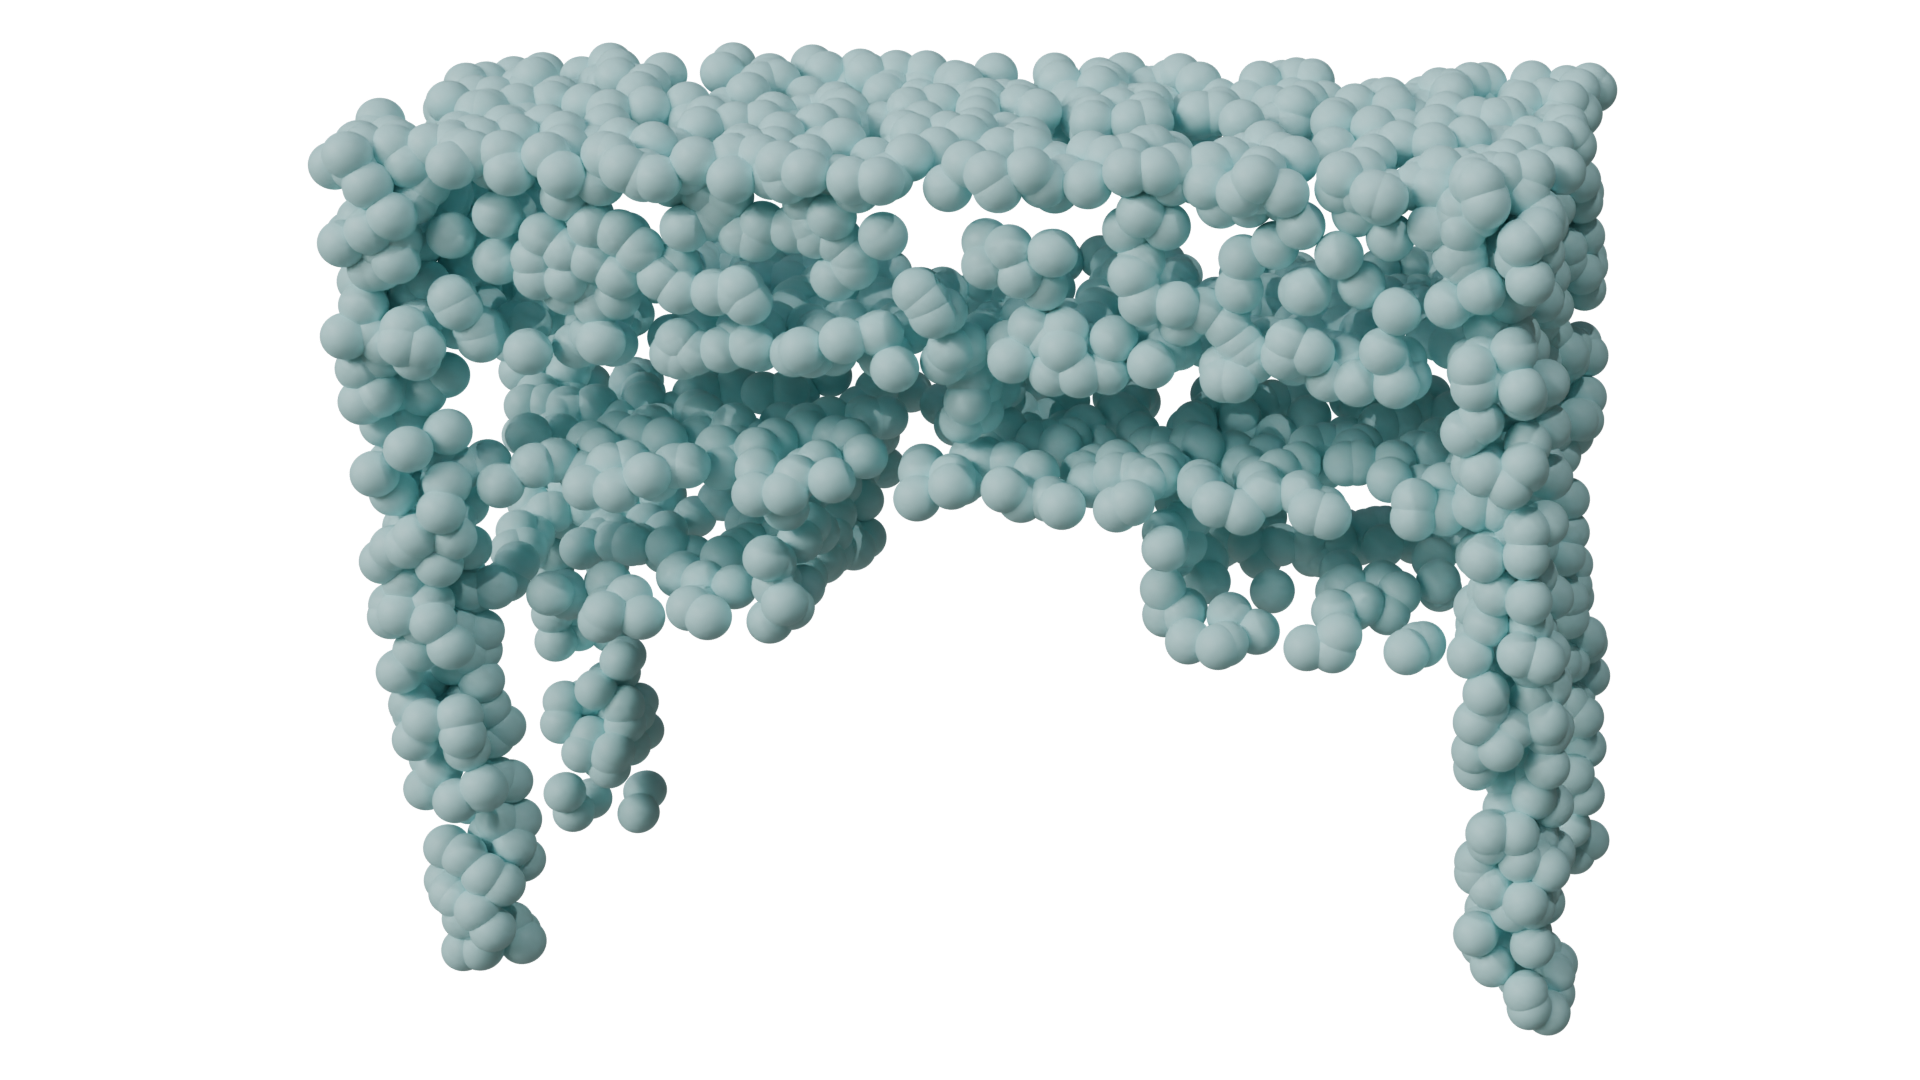
\includegraphics[width=\linewidth]{figures/gp/t1cgp.png}
    \caption{Recon 2}
\end{subfigure}
\caption{Surface reconstructions from implicit functions modeled by Gaussian process posterior mean and posterior mean $\pm$ standard deviation overlayed to see the extent to which the 3D object can cover space.}
\label{fig:one-std-gp}
\end{figure}

\begin{figure}[htb]
\centering
\begin{subfigure}{0.45\textwidth}
    \vspace{-20pt}
    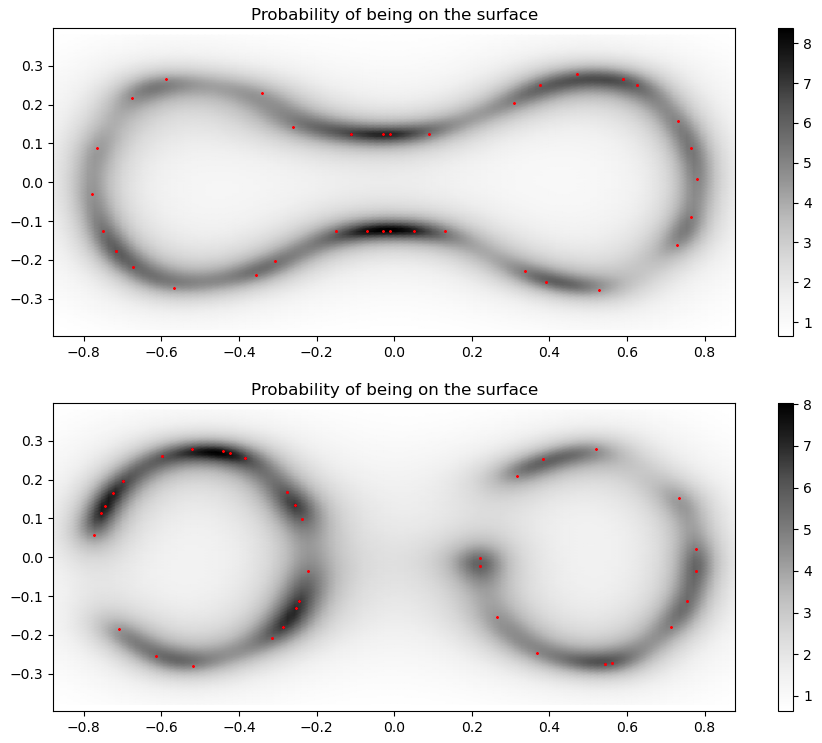
\includegraphics[width=\linewidth]{figures/gp2d/data_mapping_combined.png}
\end{subfigure}
\hfill
\begin{subfigure}{0.45\textwidth}
    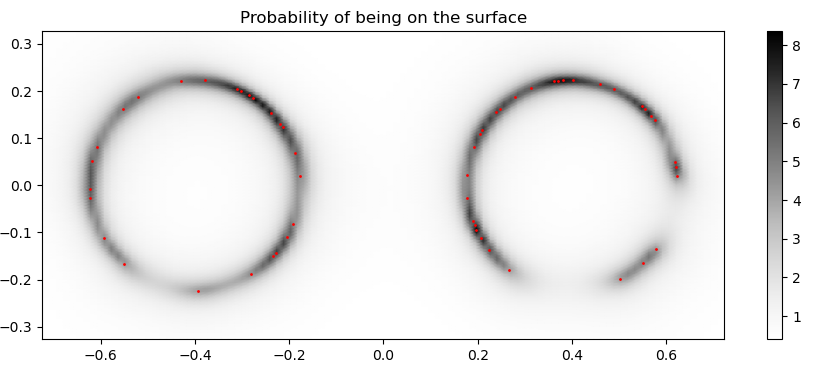
\includegraphics[width=\linewidth]{figures/gp2d/augeye.png}
    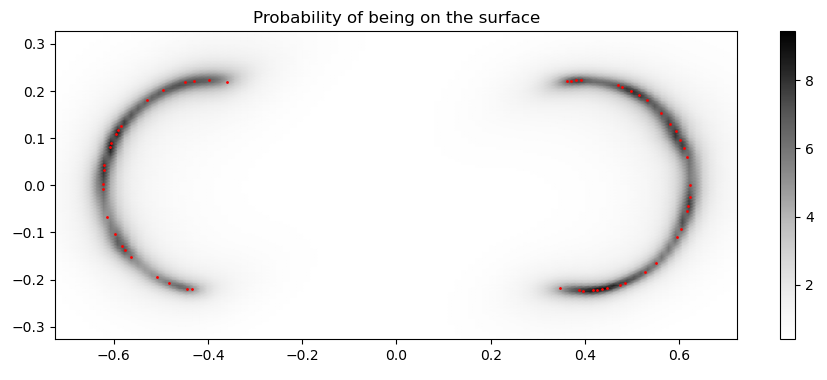
\includegraphics[width=\linewidth]{figures/gp2d/augside.png}
\end{subfigure}
\hfill
\caption{Probabilistic surface estimation in 2D using Gaussian process with posterior log-likelihood maximization of manifold points. A toy dataset of point sets from a dumbbell and two circles was used to perform this experiment.}
\label{fig:2dgp}
\end{figure}


\chapter{Example Effect of Non-zero Prior Mean in GP}\label{ch:nonzerogp}
Consider two non-similar points $x_1$ and $x_2$ with $k(x_1, x_2) = 0$ for some covariance or kernel function $k$. Therefore, the covariance matrix can be written as \[\left[\begin{array}{cc}
   1 & 0 \\
   0 & 1
\end{array}\right].\]We also observe the function values at $x_1$ and $x_2$ to be $0$ and $1$, respectively. We assume a prior mean of $1$, that is $m(x)=1$. Now, consider a new point $x^*$ more similar to $x_1$ than $x_2$, such that $k(x^*, x_1)=0.9, k(x^*, x_2)=0.1$. Then from Eq~\ref{GPPosterior}, we can compute the posterior mean at $x^*$ given $\mathbf{X}=[x_1, x_2]^T$ as:
{\small\begingroup
\renewcommand{\arraystretch}{1.25}
\setlength\arraycolsep{2.5pt}
\begin{align}
    m\left(x^*\right)+k\left(x^*, \mathbf{X}\right) k\left(\mathbf{X}, \mathbf{X}\right)^{-1}\left(\mathbf{Y}-m\left(\mathbf{X}\right)\right) & = 1 + [0.9 \hspace{5pt} 0.1] \left[\begin{array}{cc}
        1 & 0 \\
        0 & 1
    \end{array}\right]^{-1} \left(\left[\begin{array}{c}
        0\\
        1
        \end{array}\right] -
        \left[\begin{array}{c}
        1\\
        1
        \end{array}\right]
        \right)\\
        &= 1 + [0.9 \hspace{5pt} 0.1] \left[\begin{array}{cc}
        1 & 0 \\
        0 & 1
    \end{array}\right] \left[\begin{array}{c}
        -1\\
        0
        \end{array}\right]\\
        &= 1 + [0.9 \hspace{5pt} 0.1] \left[\begin{array}{c}
        -1\\
        0
        \end{array}\right]\\
        &= 1 + 0.9\cdot (-1) + 0.1 \cdot 0\\
        &= 1 -0.9\\
        &= 0.1,
\end{align}
\endgroup
}
which is close to $0$ as expected since $x^*$ is similar to $x_1$ where the function value is $0$.

Now, if we consider another point $\hat{x}$ close to $x_2$, such that $k(\hat{x}, x_1)=0.05$ and $k(x^*, x_2)=0.95$. Then from Eq~\ref{GPPosterior}, we can compute the posterior mean at $x^*$ given $\mathbf{X}=[x_1, x_2]^T$ as:
{\small\begingroup
\renewcommand{\arraystretch}{1.25}
\setlength\arraycolsep{2.5pt}
\begin{align}
    m\left(\hat{x}\right)+k\left(\hat{x}, \mathbf{X}\right) k\left(\mathbf{X}, \mathbf{X}\right)^{-1}\left(\mathbf{Y}-m\left(\mathbf{X}\right)\right) & = 1 + [0.05 \hspace{5pt} 0.95] \left[\begin{array}{cc}
        1 & 0 \\
        0 & 1
    \end{array}\right]^{-1} \left(\left[\begin{array}{c}
        0\\
        1
        \end{array}\right] -
        \left[\begin{array}{c}
        1\\
        1
        \end{array}\right]
        \right)\\
        &= 1 + [0.05 \hspace{5pt} 0.95] \left[\begin{array}{cc}
        1 & 0 \\
        0 & 1
    \end{array}\right] \left[\begin{array}{c}
        -1\\
        0
        \end{array}\right]\\
        &= 1 + [0.05 \hspace{5pt} 0.95] \left[\begin{array}{c}
        -1\\
        0
        \end{array}\right]\\
        &= 1 + 0.05\cdot (-1) + 0.95 \cdot 0\\
        &= 1 -0.05\\
        &= 0.95,
\end{align}
\endgroup
}
which is close to $1$ as expected since $\hat{x}$ is similar to $x_2$ where the observed function value is $1$.

%\index{VAEBM}
